\documentclass{article}
\usepackage{bm}
\usepackage{amsmath}
\usepackage{graphicx}
\usepackage{mdwlist}
\usepackage[colorlinks=true]{hyperref}
\usepackage{geometry}
\usepackage{kotex}
\geometry{margin=1in}
\geometry{headheight=2in}
\geometry{top=2in}
\usepackage{palatino}
%\renewcommand{\rmdefault}{palatino}
\usepackage{fancyhdr}

\newcommand{\red}[1]{{\color{red} #1}}
\newcommand{\blue}[1]{{\color{blue} #1}}
\newcommand{\orange}[1]{{\color{orange} #1}}
\newcommand{\purple}[1]{{\color{purple} #1}}

%\pagestyle{fancy}
\rhead{}
\lhead{}
\chead{%
  {\vbox{%
      \vspace{2mm}
      \large
      Hardware System Design 4190.309A\hfill
\\
      Seoul National University
      \\[4mm]
      \textbf{Practice \#7. How to use FPGA board}\\
      \textbf{Jiwon Lee, Sangjun Son}
    }
  }
}

%%%%%%%%%%%%%%%%%%%%%%%
\usepackage{xcolor}
\usepackage{listings}
\definecolor{vgreen}{RGB}{104,180,104}
\definecolor{vblue}{RGB}{49,49,255}
\definecolor{vorange}{RGB}{255,143,102}

\lstdefinestyle{verilog-style}
{
    language=Verilog,
    basicstyle=\scriptsize\ttfamily,
    keywordstyle=\color{vblue},
    identifierstyle=\color{black},
    commentstyle=\color{vgreen},
    numbers=left,
    numberstyle=\tiny\color{black},
    numbersep=10pt,
    tabsize=8,
    moredelim=*[s][\colorIndex]{[}{]},
    literate=*{:}{:}1
}

\makeatletter
\newcommand*\@lbracket{[}
\newcommand*\@rbracket{]}
\newcommand*\@colon{:}
\newcommand*\colorIndex{%
    \edef\@temp{\the\lst@token}%
    \ifx\@temp\@lbracket \color{black}%
    \else\ifx\@temp\@rbracket \color{black}%
    \else\ifx\@temp\@colon \color{black}%
    \else \color{vorange}%
    \fi\fi\fi
}
\makeatother

\usepackage{trace}
%%%%%%%%%%%%%%%%%%%%%%%

\usepackage{paralist}

\usepackage{todonotes}
\setlength{\marginparwidth}{2.15cm}

\usepackage{tikz}
\usetikzlibrary{positioning,shapes,backgrounds}

\begin{document}

\pagestyle{fancy}

\section*{Goal}

\begin{itemize*}
\item ZED Board Tutorial.
\begin{itemize*}
\item Setup the board.
\item \textit{SW2LED} module: A combinational logic that blinks \texttt{[7:0]LED} in response to \texttt{[7:0]SWITCH}.
\end{itemize*}
\item Implement a simple sequential logic with external clock.
\end{itemize*}

\begin{figure}[ht]
	\centering
	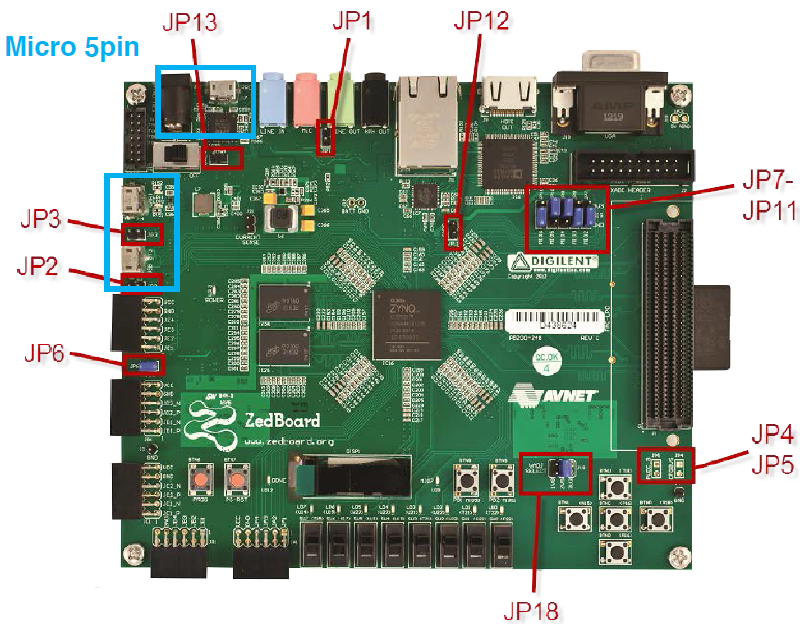
\includegraphics[width=0.75\textwidth]{fig/fig1.png}
\caption{ZedBoard Jumper Map~\cite{lab7}.}
\label{fig1}
\end{figure}

\section{Implementation}
이번 프로젝트는 ZED Board를 처음으로 수령하고 PC에 연결하여 각각의 컴포넌트를 조작할 수 있는 환경설정을 목표로 한다.
이전 Lab 세션에서는 Design과 Simulation을 통해 Verilog 코드를 작성하고 테스트 벤치 상에서 알맞는 동작을 하는지 간접적으로 확인하는 작업을 해왔다. 
이번에는 Synthesis와 Implementation을 한 이후에 Board에 Bitstream Generator를 이용해 실질적으로 올바른 동작을 하는지 눈으로 확인할 수 있을 것이다.
튜터리얼로 토글된 스위치에 해당하는 위치의 LED가 켜지는 프로그램을 통해 보드의 컴포넌트 작동을 확인하고 이후 실습으로 \textit{1 sec Checker}를 구현하고 이를 보드 위에서 잘 작동하는지 확인할 것이다.

\subsection{ZED Board Tutorial}
8 switches와 8 LEDs를 서로 연결하는 코드는 다음과 같으며 보드에 해당하는 컴포넌트 번호는 Hardware User's Guide~\cite{UG}를 참고하였다. 기존 프로젝트와는 다르게 User Constraints를 작성해주어야 하며 이는 제공된 템플릿을 활용해 원하는 포트 및 전달받을 신호 변수를 지정해주었다.

\subsubsection*{\textit{SW2LED}}

\begin{itemize*}
\item Verilog Code, \texttt{sw2led.v}
\begin{lstlisting}[style={verilog-style}]
`timescale 1ns / 1ps
module sw2led(
    input [7:0] SW,
    output [7:0] LD
    );
    assign LD = SW;
    
endmodule
\end{lstlisting}

\item User Constraints, \texttt{sw2led.xdc}
\begin{lstlisting}[style={verilog-style}]
# ----------------------------------------------------------------------------
# User DIP Switches - Bank 35
# ---------------------------------------------------------------------------- 
set_property PACKAGE_PIN F22 [get_ports {SW[0]}];  # "SW0"
set_property PACKAGE_PIN G22 [get_ports {SW[1]}];  # "SW1"
set_property PACKAGE_PIN H22 [get_ports {SW[2]}];  # "SW2"
set_property PACKAGE_PIN F21 [get_ports {SW[3]}];  # "SW3"
set_property PACKAGE_PIN H19 [get_ports {SW[4]}];  # "SW4"
set_property PACKAGE_PIN H18 [get_ports {SW[5]}];  # "SW5"
set_property PACKAGE_PIN H17 [get_ports {SW[6]}];  # "SW6"
set_property PACKAGE_PIN M15 [get_ports {SW[7]}];  # "SW7"
set_property IOSTANDARD LVCMOS25 [get_ports -of_objects [get_iobanks 35]];

# ----------------------------------------------------------------------------
# User LEDs - Bank 33
# ---------------------------------------------------------------------------- 
set_property PACKAGE_PIN T22 [get_ports {LD[0]}];  # "LD0"
set_property PACKAGE_PIN T21 [get_ports {LD[1]}];  # "LD1"
set_property PACKAGE_PIN U22 [get_ports {LD[2]}];  # "LD2"
set_property PACKAGE_PIN U21 [get_ports {LD[3]}];  # "LD3"
set_property PACKAGE_PIN V22 [get_ports {LD[4]}];  # "LD4"
set_property PACKAGE_PIN W22 [get_ports {LD[5]}];  # "LD5"
set_property PACKAGE_PIN U19 [get_ports {LD[6]}];  # "LD6"
set_property PACKAGE_PIN U14 [get_ports {LD[7]}];  # "LD7"
set_property IOSTANDARD LVCMOS33 [get_ports -of_objects [get_iobanks 33]];
set_property IOSTANDARD LVCMOS25 [get_ports -of_objects [get_iobanks 34]];
\end{lstlisting}
\end{itemize*}

위의 모듈 코드를 보면 입력과 출력으로 8 비트 \texttt{SW}와 \texttt{LD}가 있는 것을 확인할 수 있다. 단순히 두 개의 wire를 이어주는 논리로 작성이 되었으며 사용되는 입력과 출력 신호는 각각 DIP Switches (Bank 35)와 User LEDs (Bank 33)에 해당하는 컴포넌트의 포트번호를 통해 연결되어 있는 것을 확인할 수 있다~\cite{UG}.

\newpage
\subsection{Practice: One Second Checker}
One Second Checker는 크게 Down counter와 Up counter로 구성되어 있다. Down counter는 \texttt{GCLK}의 신호를 초 단위로 바꿔주는 역할을 하며 Up counter는 Down counter에 따라 즉 초 단위로 카운트가 되는 역할을 한다. Up counter를 LED에 연결하여 보드에서 확인할 수 있게 하였다.

\subsubsection*{\textit{One Second Checker}}

\begin{itemize*}
\item Verilog Code, \texttt{one\_sec\_checker.v}
\begin{lstlisting}[style={verilog-style}]
`timescale 1ns / 1ps

module one_sec_checker#(
    parameter CLK_FREQ = 28'd100000000
)(
    input GCLK,
    input BTNC,
    output [7:0] LD
    );
    
    reg [27:0] down_counter;
    reg [7:0] up_counter;
    assign LD = up_counter;
    
    initial begin
        up_counter <= 0;
        down_counter <= CLK_FREQ;
    end
    
    always @(posedge GCLK or posedge BTNC) begin
        if (BTNC) begin
            up_counter <= 0;
            down_counter <= CLK_FREQ;
        end
        else begin
            if (down_counter == 0) begin
                up_counter <= up_counter + 8'd1;
                down_counter <= CLK_FREQ;
            end
            else begin
                down_counter <= down_counter - 28'd1;
            end
        end
    end
endmodule
\end{lstlisting}

\item User Constraints, \texttt{one\_sec\_checker.xdc}
\begin{lstlisting}[style={verilog-style}]
# ----------------------------------------------------------------------------
# Clock Source - Bank 13
# ---------------------------------------------------------------------------- 
set_property PACKAGE_PIN Y9 [get_ports {GCLK}];  # "GCLK"
set_property IOSTANDARD LVCMOS33 [get_ports -of_objects [get_iobanks 13]];

# ----------------------------------------------------------------------------
# User LEDs - Bank 33
# ---------------------------------------------------------------------------- 
set_property PACKAGE_PIN T22 [get_ports {LD[0]}];  # "LD0"
set_property PACKAGE_PIN T21 [get_ports {LD[1]}];  # "LD1"
set_property PACKAGE_PIN U22 [get_ports {LD[2]}];  # "LD2"
set_property PACKAGE_PIN U21 [get_ports {LD[3]}];  # "LD3"
set_property PACKAGE_PIN V22 [get_ports {LD[4]}];  # "LD4"
set_property PACKAGE_PIN W22 [get_ports {LD[5]}];  # "LD5"
set_property PACKAGE_PIN U19 [get_ports {LD[6]}];  # "LD6"
set_property PACKAGE_PIN U14 [get_ports {LD[7]}];  # "LD7"
set_property IOSTANDARD LVCMOS33 [get_ports -of_objects [get_iobanks 33]];

# ----------------------------------------------------------------------------
# User Push Buttons - Bank 34
# ---------------------------------------------------------------------------- 
set_property PACKAGE_PIN P16 [get_ports {BTNC}];  # "BTNC"
set_property IOSTANDARD LVCMOS25 [get_ports -of_objects [get_iobanks 34]];
\end{lstlisting}
\end{itemize*}

\begin{figure}[htb!]
	\centering
	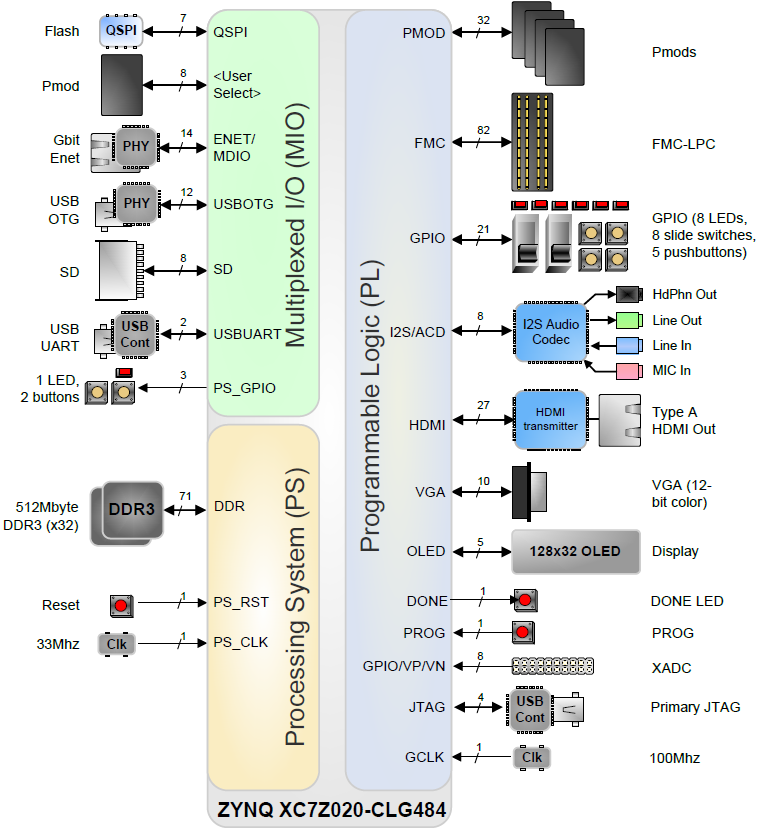
\includegraphics[width=0.6\textwidth]{fig/fig2.png}
\caption{ZedBoard Block Diagram~\cite{UG}.}
\label{fig2}
\end{figure}

ZedBoard의 Clock frequency를 확인하기 위해서 User Guide에 적힌 스펙을 확인하면 된다. Figure~\ref{fig2}에서 볼 수 있듯이 \texttt{GCLK}은 100 MHz의 주기를 가지므로 Down counter를 $\texttt{CLK\_FREQ}=10^8$으로 초기화 한다. 그리고 매 \texttt{GCLK} 신호 마다 counter에서 1을 빼주는 방식으로 업데이트 해준다.
Down counter가 0이 됐다면 이는 1초가 흘렸음을 의미하고 Up counter (1초마다 증가하는 카운터)에 1을 증가시키고 동시에 Down counter를 다시 $\texttt{CLK\_FREQ}=10^8$으로 초기화 한다. 이때 리셋 신호인 \texttt{BTNC} 신호가 들어오면 Clock 신호에 Asynchronous하게 Down counter, Up counter 모두 초기화 해준다. \\

위의 User Constraints는 입력 \texttt{GCLK}, \texttt{BTNC}와 출력 \texttt{LD}에 해당하는 포트에 대응되는 환경 변수를 표현한 코드이. 각각 Clock Source (Bank 13), User Push Buttons (Bank 34) 와 User LEDs (Bank 33)에 해당하는 컴포넌트의 포트번호를 통해 연결되어 있는 것을 확인할 수 있다~\cite{UG}.

\newpage
\section{Experiments}

\subsection{Implementation Results}

\begin{figure}[htb!]
	\centering
	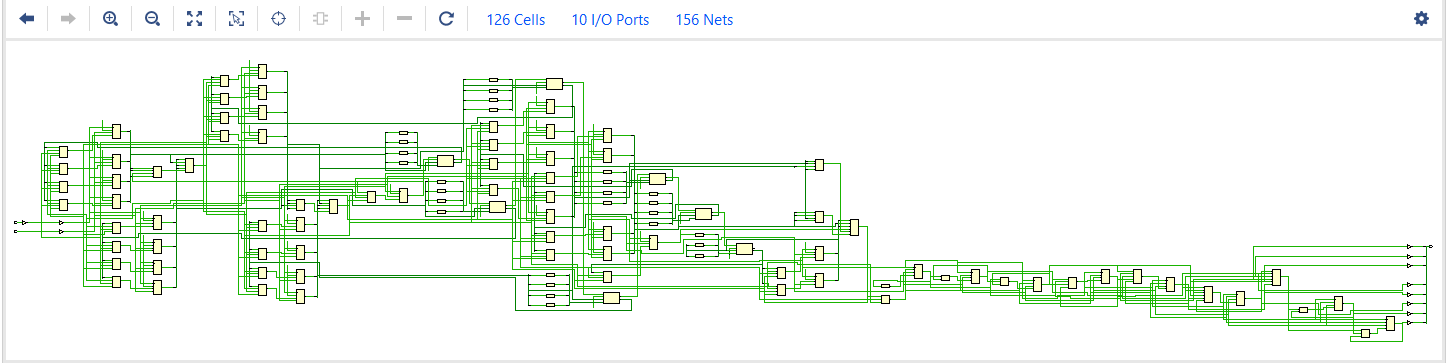
\includegraphics[width=1\textwidth]{fig/Schematic.png}
\caption{Schematic of \textit{One Second Checker} after Implementation}
\label{schematic}
\end{figure}
\begin{figure}[htb!]
	\centering
	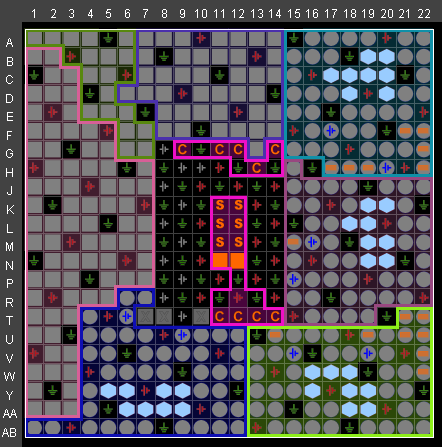
\includegraphics[width=0.4\textwidth]{fig/IO.png}
\caption{I/O ports used in \textit{One Second Checker} after Implementation}
\label{io}
\end{figure}

\newpage
\subsection{Execution Results}

\begin{figure}[htb!]
	\centering
	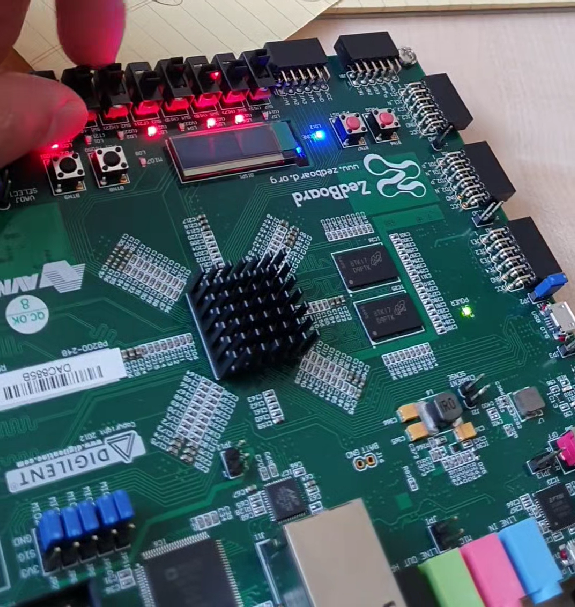
\includegraphics[width=0.45\textwidth]{fig/sw2led.png}
	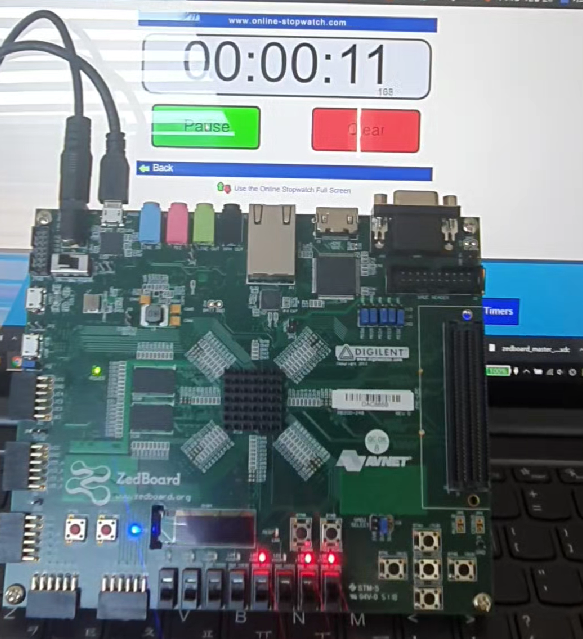
\includegraphics[width=0.45\textwidth]{fig/one_sec_checker.png}
\caption{Execution results of \textit{SW2LED} and \textit{One Second Checker}}
\label{execution}
\end{figure}

\section{Conclusion}
이번 주 실습 결과는 영상으로 촬영하여 압축파일에 함께 첨부하였다.
이번 실습은 구현 사항에 있어서는 그렇게 어려운 부분은 없었지만 기존의 실습과는 다르게 환경을 제대로 설정해주어야 원하는 결과를 얻을 수 있다는 것을 확인하였다. \\

Verilog 코드의 Port와 보드의 구성품과 연결하고 올바르게 전압을 올려줘야 하는 과정에서 혼란을 겪었고 앞으로의 실습에서도 사소한 구현이 동작여부를 좌지우지할 수 있을 것이라는 우려를 낳았다. ZedBoard User Guide~\cite{UG}를 자주 참고할 것 같다. Synthesis, Implementation 그리고 Bitstream Generation을 수행하는데 오랜 시간이 걸리는 만큼 Simulation test bench의 중요성 또한 상기하였다.\\

\bibliographystyle{plain}
\bibliography{other}

\end{document}
